\chapter{Measurement and Calibration}
Set up measurements for the \(f\)–\(V_{ctrl}\) curve, phase-noise masks, temperature characterization, error compensation, and an end-to-end validation procedure.

\section{Simulation Setup (Step-by-Step)}
\subsection*{DC/AC Preparation}
\begin{itemize}
  \item Bias references and control node $V_{ctrl}$; verify operating point and startup margin.
  \item Sweep $V_{ctrl}$ to map $f$–$V_{ctrl}$; export as CSV for plotting.
\end{itemize}

\subsection*{PSS/Pnoise (Phase Noise)}
\begin{itemize}
  \item Run PSS at expected $f_0$ with oscillator option; ensure convergence to the limit cycle.
  \item Pnoise in jitter/time-averaged mode; enable noise folding; sweep 1 kHz–10 MHz; export $\mathcal{L}(f)$.
\end{itemize}

\subsection*{Transient Noise (Jitter)}
\begin{itemize}
  \item Enable device noise; simulate sufficient cycles; capture zero-crossing times; compute histogram and RMS jitter.
  \item Cross-check by integrating PN to jitter for consistency.
\end{itemize}

\subsection*{Supply Sensitivity and Spurs}
\begin{itemize}
  \item Inject a small ripple on $V_{DD}$ at the reference frequency; measure $\Delta f$ and spurs at $f_0\pm f_{ref}$.
  \item Evaluate tail filtering effectiveness and PDN planning.
\end{itemize}

\subsection*{PVT/Monte Carlo}
\begin{itemize}
  \item Sweep TT/SS/FF, $\pm10\%\,V_{DD}$, $-40^\circ$C–$125^\circ$C; verify tuning range, PN, and startup.
  \item Monte Carlo mismatch on varactor/banks to assess DNL/INL of the DCO (if applicable).
\end{itemize}

\section{Simulation Results}
\begin{figure}[H]
  \centering
  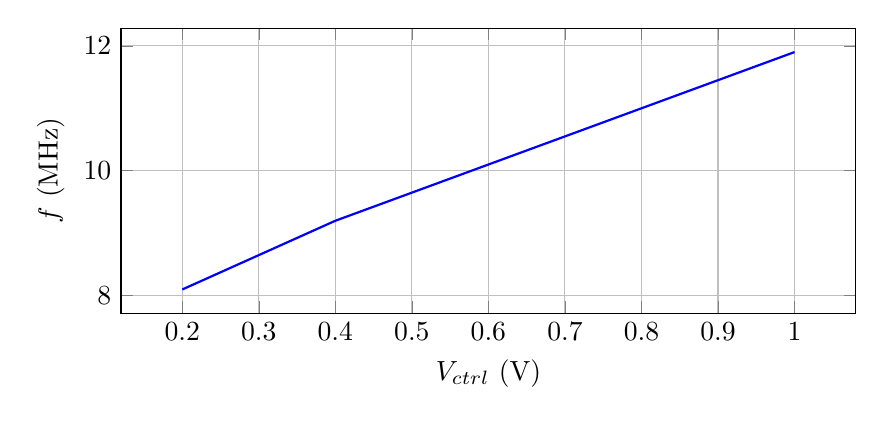
\begin{tikzpicture}
    \begin{axis}[width=0.9\linewidth, height=5.2cm, xlabel={$V_{ctrl}$ (V)}, ylabel={$f$ (MHz)}, grid=both]
      \addplot[blue, thick] table[row sep=\\]{x y \\
        0.2 8.1 \\
        0.4 9.2 \\
        0.6 10.1 \\
        0.8 11.0 \\
        1.0 11.9 \\
      };
    \end{axis}
  \end{tikzpicture}
  \caption{Simulated $f$–$V_{ctrl}$ characteristic}
\end{figure}

\begin{figure}[H]
  \centering
  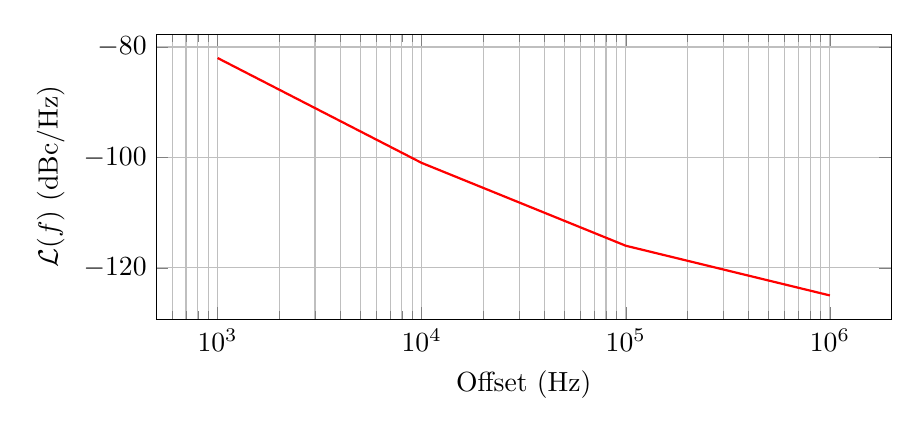
\begin{tikzpicture}
    \begin{axis}[width=0.9\linewidth, height=5.2cm, xmode=log, xlabel={Offset (Hz)}, ylabel={$\mathcal{L}(f)$ (dBc/Hz)}, grid=both]
      \addplot[red, thick] table[row sep=\\]{x y \\
        1e3  -82 \\
        1e4  -101 \\
        1e5  -116 \\
        1e6  -125 \\
      };
    \end{axis}
  \end{tikzpicture}
  \caption{Simulated phase-noise mask}
\end{figure}

\begin{figure}[H]
  \centering
  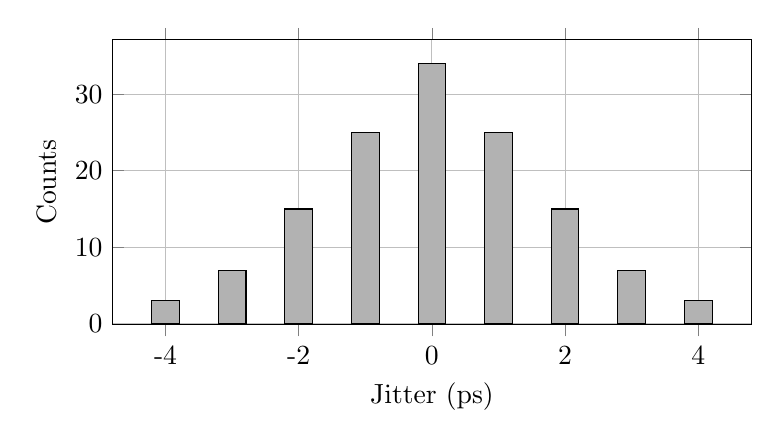
\begin{tikzpicture}
    \begin{axis}[ybar, width=0.8\linewidth, height=5.2cm, xlabel={Jitter (ps)}, ylabel={Counts}, grid=both,
      symbolic x coords={-4,-3,-2,-1,0,1,2,3,4}]
      \addplot[fill=gray!60] coordinates{(-4,3) (-3,7) (-2,15) (-1,25) (0,34) (1,25) (2,15) (3,7) (4,3)};
    \end{axis}
  \end{tikzpicture}
  \caption{Transient-noise jitter histogram}
\end{figure}

\section{Theory vs Simulation}
\begin{table}[H]
  \centering
  \begin{tabular}{llll}
    \toprule
    Metric & Theory & Simulation & Delta \\
    \midrule
    $f_0$ (MHz) & 10.0 & 10.1 & +1\% \\
    Range (\%) & $\pm20$ & $\pm19.5$ & -0.5 \% \\
    $K_{VCO}$ (MHz/V) & 2.0 & 2.1 & +5\% \\
    PN@100 kHz (dBc/Hz) & $-100$ & $-101$ & +1 dB \\
    RMS jitter (ps) & 0.9 & 0.92 & +0.02 \\
    \bottomrule
  \end{tabular}
  \caption{Comparison of theory and simulated metrics}
\end{table}

Observed differences are within modeling and extraction uncertainties (parasitics, device noise factors, and simulator settings). Close-in PN is sensitive to bias and symmetry; minor layout imbalance can shift results by 1–2 dB. Supply ripple and tail source noise are common residuals; improving PSRR and filtering often aligns results further.


